% figure: 现控强化2-20-正确状态变量图.png
\documentclass[border=12pt]{standalone}
\usepackage{fontspec}
\setmainfont{Cambria}
\usepackage{unicode-math}
\setmathfont{Cambria Math}
\usepackage{tikz}
\usetikzlibrary{arrows.meta,calc}
\begin{document}
\begin{tikzpicture}[>=Stealth,line width=.9pt,
 b/.style={draw,minimum width=1cm,minimum height=.8cm,fill=blue!4},
 s/.style={draw,circle,minimum size=.44cm,inner sep=0pt}]
\node[s] (s1) at (0,0) {$+$};
\node[b] (i1) at (2,0) {$\dfrac{1}{s}$};
\node[s] (s2) at (4,0) {$+$};
\node[b] (i2) at (6,0) {$\dfrac{1}{s}$};
\node[s] (sy) at (8,0) {$+$};
\node[b] (g2) at (6,-1.8) {$-2$};
\node[b] (g1) at (3,-3.3) {$-2$};
\draw[->] (-1.4,0) -- node[above] {$v$} (s1);
\draw[->] (s1) -- node[above] {$\dot x_1$} (i1);
\draw[->] (i1) -- node[pos=.3,above] {$x_1$} (s2);
\draw[->] (s2) -- node[above] {$\dot x_2$} (i2);
\draw[->] (i2) -- node[pos=.3,above] {$x_2$} (sy);
\draw[->] (sy) -- node[above] {$y$} (9.4,0);
\fill (3.15,0) circle(1.4pt);
\draw[->] (3.15,0) -- (3.15,1.6) -| (sy.north);
\fill (7.15,0) circle(1.4pt);
\draw[->] (7.15,0) |- (g2.east);
\draw[->] (g2.west) -| (s2.south);
\fill (7.15,-1.8) circle(1.4pt);
\draw[->] (7.15,-1.8) |- (g1.east);
\draw[->] (g1.west) -| (s1.south);
\end{tikzpicture}
\end{document}
